\documentclass[12pt]{article}
\usepackage{hyperref}
\usepackage{listings}
\usepackage[margin=1in]{geometry}
\usepackage{enumitem}
\usepackage{multicol}
\usepackage{array}
\usepackage{titlesec}
\usepackage{helvet}
\renewcommand{\familydefault}{\sfdefault}
\usepackage{amsmath}     % For math equations
\usepackage{amssymb}     % For advanced math symbols
\usepackage{amsfonts} % For math fonts
\usepackage{gvv}
\usepackage{esint}
\usepackage[utf8]{inputenc}
\usepackage{graphicx}
\usepackage{pgfplots}
\pgfplotsset{compat=1.18}
\titleformat{\section}{\bfseries\large}{\thesection.}{1em}{}
\setlength{\parindent}{0pt}
\setlength{\parskip}{6pt}
\usepackage{multirow}
\usepackage{float}
\usepackage{caption}


\begin{document}
    



\newpage
\begin{center}
\textbf{\Large AI25BTECH11034 - SUJAL CHAUHAN }\\
\textbf {2.7.6}
\end{center}
\textbf{question}\\
find the area of triangle with vertices (2,0), (1,4), (4,5) 
\begin{center}
\begin{tabular}{|c|c|}
\hline
Points & Vector \\ \hline
$\Vec{A}$ & $\myvec{2 \\ 0}$\\ \hline
$\Vec{B}$ & $\myvec{4 \\ 5}$\\ \hline
$\Vec{C}$ & $\myvec{1\\ 4}$\\ \hline

\end{tabular}
\end{center}

\begin{align}
    \vec{A}-\vec{B}=\myvec{-2 \\ -5}
\end{align}
\begin{align}
    \vec{A}-\vec{C}=\myvec{1\\-4}
\end{align}
Area of triangle formed by the given points
\begin{align}
    \frac{1}{2}\norm{(\Vec{A}-\Vec{B})\times(\Vec{A}-\Vec{C})}=\frac{13}{2}
\end{align}
Area of formed by the given points is $\frac{13}{2}$
 square units.
\newpage
\begin{figure}[h]
    \centering
    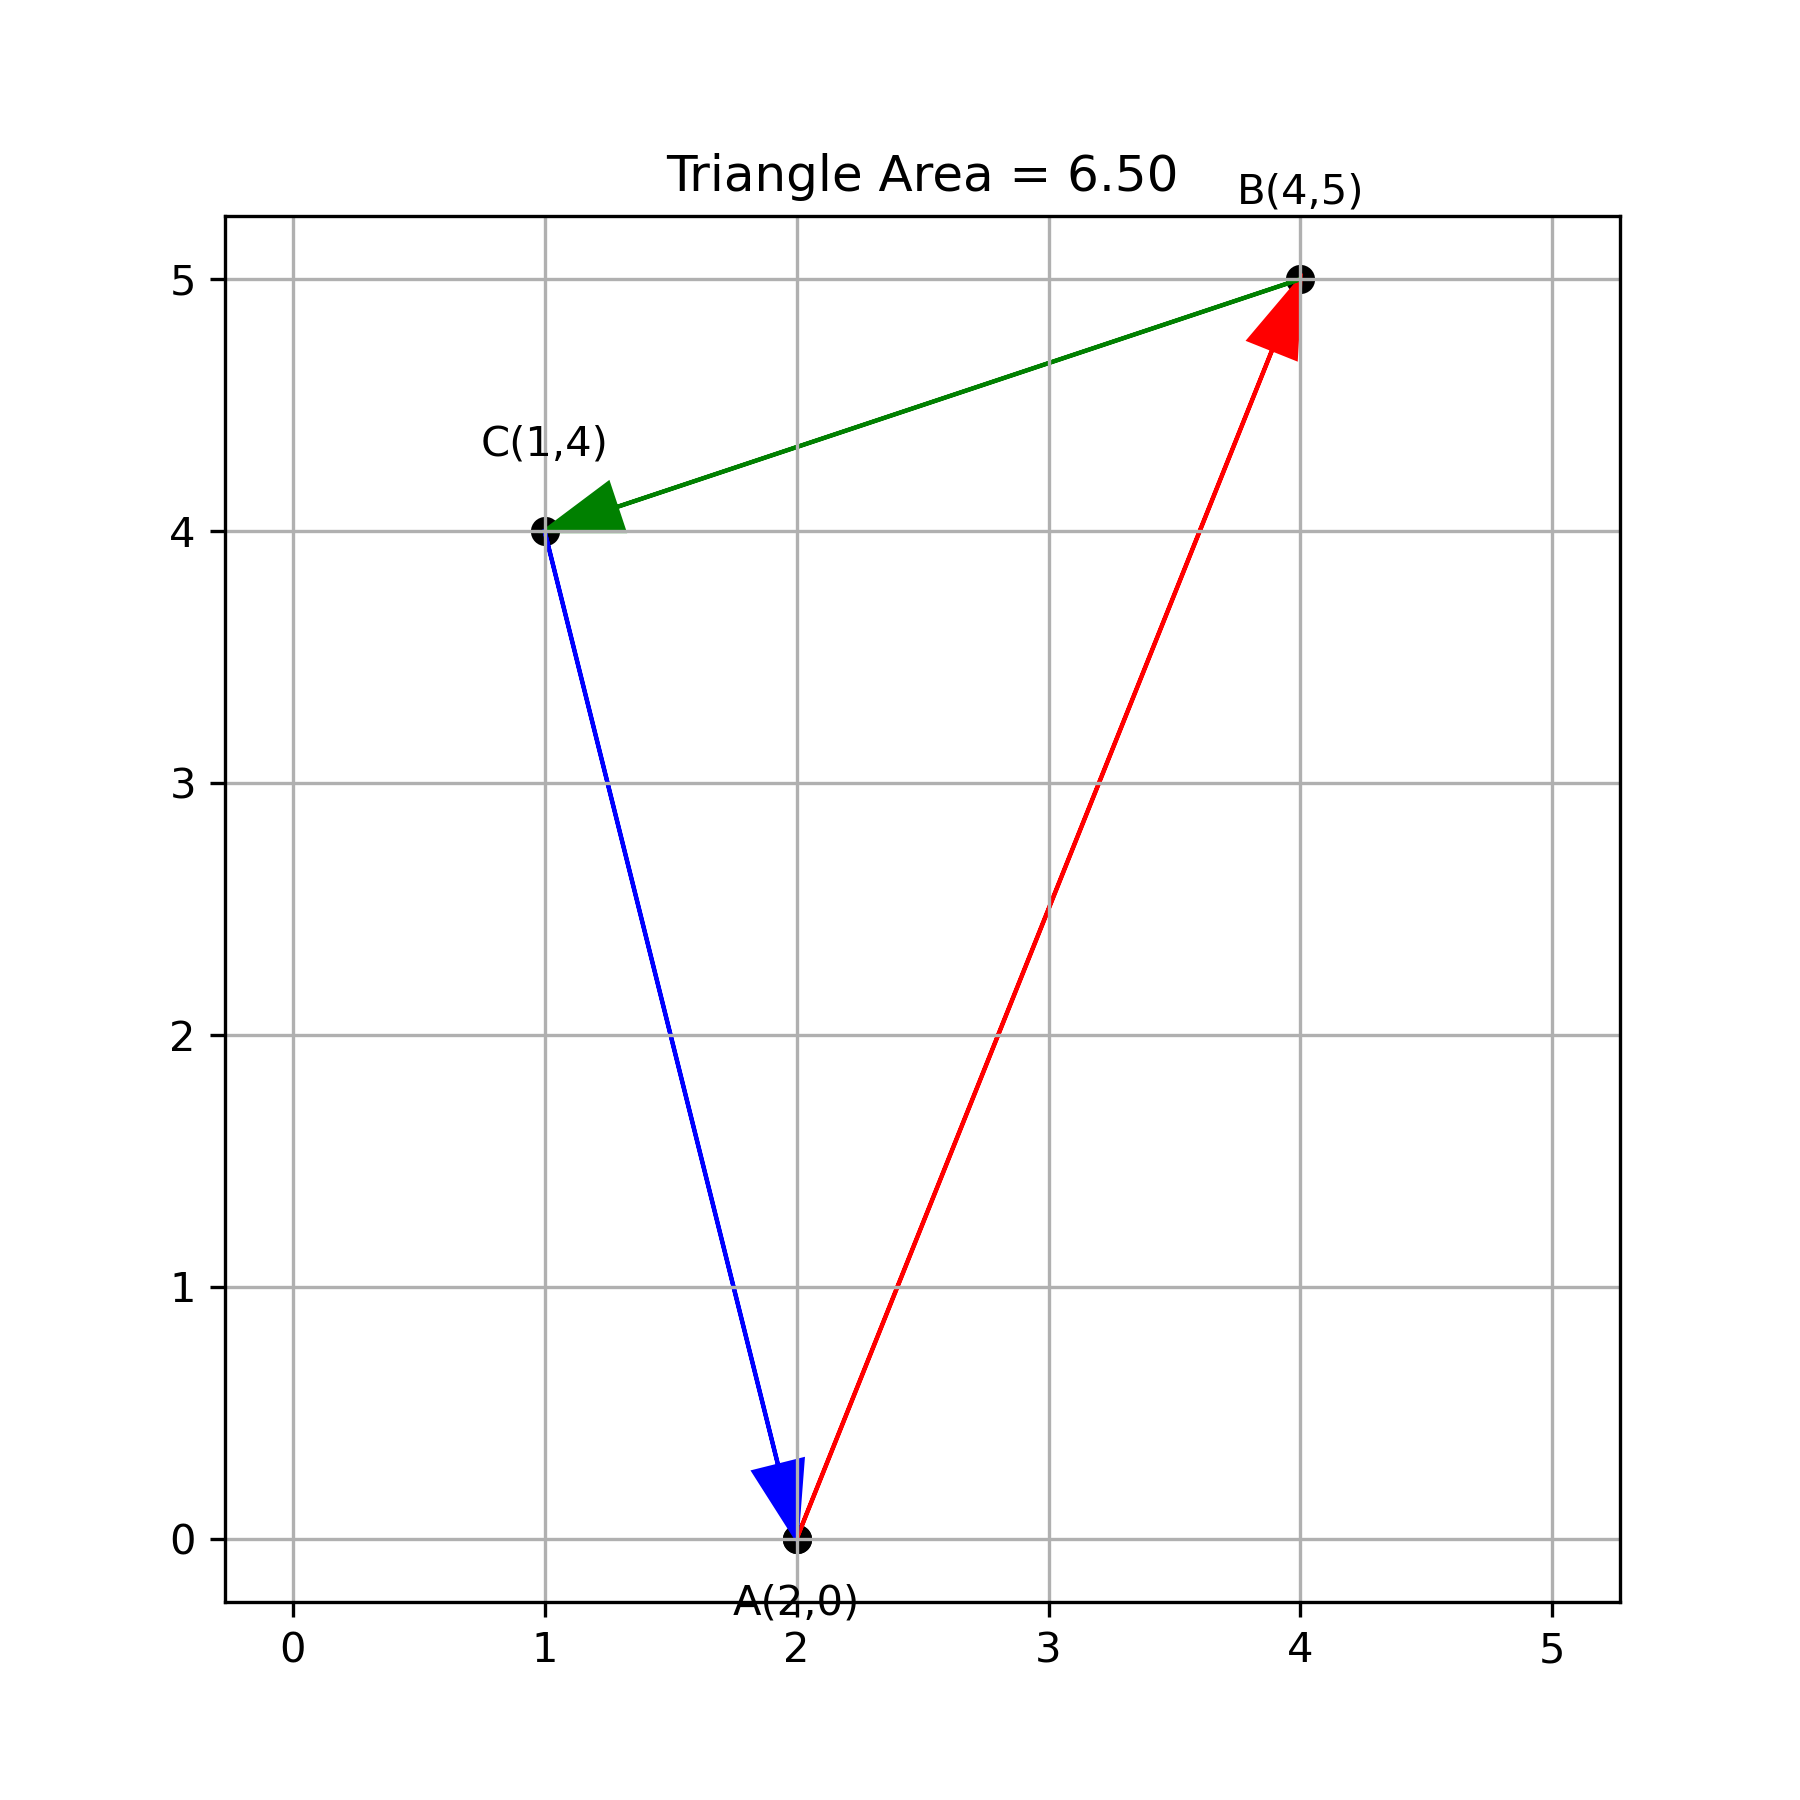
\includegraphics[width=0.5\linewidth]{figures/triangle.png}
    \caption{Caption}
    \label{fig:placeholder}
\end{figure}




\end{document}
